\section{Battery Rack}
The battery rack in the robot located right above the motors in the frame. The number of batteries required for the operation of the robot is six batteries and the frame gave just enough room for the structure of the battery rack and the batteries themselves. The reason for the size batteries is because two are required to be connected in series to supply the controller with enough voltage to be split and supplying each motor with 25 volts. The proposal design of the battery rack to consist of 2"x2"x1/8" aluminum tubing but since Penguin ASI requested to use their spare material the tubing that was used was 2"x2"x1/4" aluminum tubing. The batteries are located at a height is near the top of the chassis which allowed the installer to have an easier job of placing the batteries in the frame from the original design. Since in the original design the installer had to place the batteries at the base of the frame which would put the installer at risk of injury. 
\subsection{Design Constraints}
The size of battery rack was constrained to the chassis that was provided. the available room that for the batteries in the frame was 1.82 m by 0.73 m. With this area six batteries were able to be placed in the frame in an orientation that had them all in line as can be seen in Figure~\ref{fig:battery_rack_section}.
\begin{figure}[htbp]
	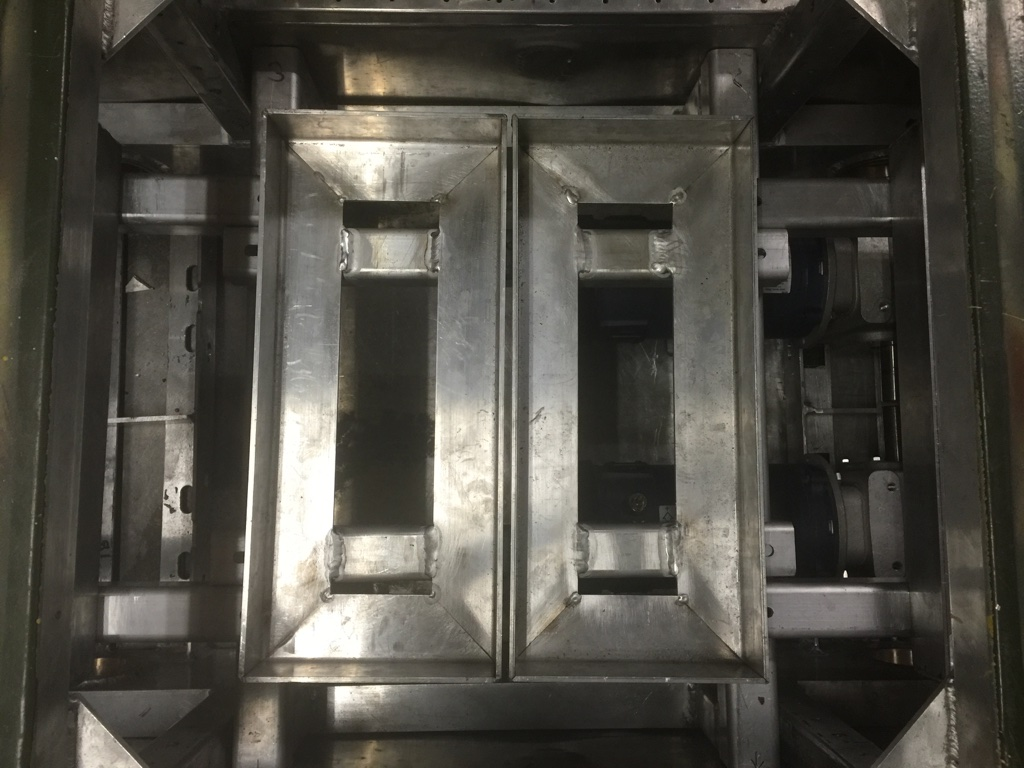
\includegraphics[width=\linewidth]{images/battery_rack_mid_bld.jpg}
	\caption{One section of three of the battery rack.}
	\label{fig:battery_rack_section}
\end{figure}
\subsection{Functional Requirements}
\subsection{Analysis and Design}
\subsubsection{Battery Mounts}
\subsubsection{Battery Support Frame}
